\chapter{Technische Umsetzungen}
\label{chap:technologies}

\section{DNSSEC}
\label{sec:tec-dnssec}
DNSSEC, als eine Sammlung an IETF-Spezifikationen, erweitert DNS mit dem Ziel die Integrität und Authentizität der Ressourceneinträge sicherzustellen \cite{Arends2005}. Dies wird über die kryptografische Signatur der Einträge erreicht. Die Signaturen werden pro RRSet in eigenen RR vom Typ RRSIG gespeichert und den Antworten beigefügt. Zur Validierung wird eine Chain-Of-Trust (siehe Abschnitt \ref{sec:trust}) genützt, die ihren Ankerpunkt in einem \ac{DNSSEC}-Root-Key besitzt, welcher von der ICANN veröffentlicht wird. Der Umstand, dass die ICANN somit als alleinige Kontrollinstanz (Single-Point-Of-Trust) fungiert, wird teils als Verletzung des Grundgedanken eines verteilten, unabhängigen Internets verstanden \cite{Finch2014}.
Abgesehen davon findet die Erweiterung, aufgrund der langen Entwicklungszeit, der (verglichen zum DNS-Protokoll) hohen Komplexität und dem erhöhtem administrativem Aufwand, nur wenig Anklang. Seit der finalen Veröffentlichung 2005 konnten zwar 90 Prozent der TLD-Betreibenden zum signieren ihrer Zonen bewegt werden, die Verbreitung signierter SLDs ist mit ca. 4 Prozent jedoch zu gering um Maßgeblich zur Sicherheit des globalen DNS beizutragen \cite{DCCommunications2018}. Zusätzlich wurde das Schutzziel der Vertraulichkeit bewusst unbehandelt gelassen. Wie in Abschnitt \ref{sec:thread-priv} beschrieben, ist der Bedarf nach einer vertraulichen Möglichkeit zur Auflösung von Namen im Internet stark angestiegen. Betrachtet man zusätzlich den Umstand, dass das \ac{DNSSEC}s Netzwerkprotokoll noch stärker als reines DNS, für \ac{DoS}-Amplification genützt werden kann, ist klar, warum diese Spezifikationssammlung so wenig positive Resonanz erhält \cite{Antic2014}.

\section{DNSCurve}
\label{sec:tec-dnscurve}
Aufgrund der schlechten Akzeptanz von \ac{DNSSEC} veröffentlichte der US-amerikanische Kryptograf \ac{DJB} eine eigene Lösung namens DNSCurve. Diese dient zur Sicherstellung einer vertraulichen und authentischen Kommunikation zwischen rekursiv auflösendem Server und den autoritativen Servern. Diese baut auf dem, von \ac{DJB} entwickelten, elliptische Kurven-Kryptosystem Curve25519 auf. DNSCurve verwendet, im Gegensatz zu \ac{DNSSEC}, welches RSA einsetzt, \ac{ECC} für asymmetrische Operationen. Außerdem wird der, ebenfalls selbst entwickelte, Poly1305 \ac{MAC} für die Verschlüsselung und Echtheitsprüfung der Nachrichten eingesetzt. 

Der Einsatz von \ac{ECC} sorgt, im Vergleich zu RSA, für eine signifikante Verbesserung der Performance bei der Schlüsselaushandlung. Da weit kürzere Schlüssel bei gleichbleibender Sicherheit eingesetzt werden können, werden außerdem Probleme mit übergroßen Paketen verhindert \cite{Gupta2002}. Der in RFC7905 \cite{rfc7905} spezifizierten Poly1305 Algorithmus ist ebenfalls auf Geschwindigkeit unter Einhaltung der Sicherheitsansprüche optimiert \cite{Bernstein2005}. Somit war DNSCurve bei seiner Veröffentlichung 2009 \ac{DNSSEC} überlegen. Da der höhere Leistungsanspruch der Validierung bis heute ein starkes Argument gegen den Einsatz von \ac{DNSSEC} dargestellt, wurde DNSCurve trotz der ungewöhnlichen Algorithmen positiv aufgenommen \cite{Henry2013}. Dies Überrascht, da DNSCurve, wie D. Kaminsky feststellt, ein konzeptionelles Problem im Bereich des \textit{Trust Establishment} Prozesses aufweist \cite{Kaminsky2011}. 

Das Protokoll verlässt sich beim Auffinden der öffentlichen Schlüssel auf einen speziellen NS-Eintrag, jenen zur Ziel-DNS-Domäne. Da DNSCurve ohne Erweiterungen des DNS-Protokolls auskommt, wird dieser Eintrag lediglich durch dessen spezielles Format aufgefunden. Darüber hinaus wird der Schlüssel in den NS-Eintrag selbst kodiert. Ein Angreifer in einer aktiven MITM Position (siehe \ref{sec:attack-mitm}) könnte somit, durch simples Umschreiben des Eintrags, eine Kommunikation über DNSCrypt unterbinden. Selbst wenn kein Fallback zur Klartextkommunikation erfolgt, besteht noch immer die Möglichkeit, ein eigenes Schlüsselpaar zu generieren und den öffentlichen Schlüssel des Ziels gegen diesen zu tauschen. In der Spezifikation scheint zwar die Möglichkeit zum Aufbau einer CoT auf, da eine zentrale Vertrauensinstanz bewusst fehlt, wird diese von Kaminsky als \textit{ineffektiv} bezeichnet, da sie laut ihm keine zufriedenstellende Lösung des Problems bringt. Es ist somit fraglich, ob DNSCurve  Vertraulichkeit und Authentizität von DNS sicherstellen kann.  

\section{DNSCrypt}
Zusätzlich zu DNSCurve und \ac{DNSSEC} wurde 2011 das Netzwerkprotokoll DNSCrypt entwickelt. Dieses ähnelt DNSCurve im grundlegenden Aufbau, da es die Algorithmen Curve25519 und Poly1305 verwendet und das standardkonforme DNS Netzwerkprotokoll für die Kommunikation einsetzt. Der größte Unterschied liegt darin, dass DNSCrypt die Kommunikation zwischen Stub-Resolver und rekursivem DNS Server schützt. Um dies zu erreichen werden kurzlebige Zertifikate eingesetzt, welche zur Verschlüsselung der Anfragen und Validierung der Antworten eingesetzt werden. Diese Zertifikate sind mit einem langlebigen Schlüssel signiert, wobei der öffentliche Schlüssel von jedem Client explizit in eine Liste an vertrauenswürdigen Schlüsseln aufgenommen werden muss \cite{Denis2016}. Dies umgeht zwar die konzeptionelle Schwäche von DNSCrypt, ist jedoch ohne entsprechende Unterstützungsmethoden nicht praktikabel. Eine in manchen Implementierungen verwendete Lösung nach dem \ac{TOFU} Prinzip wird als nicht zuverlässig erachtet \cite{Wendlandt2008}. 

Somit stellt DNSCrypt, ähnlich wie DNSCurve, zwar eine sichere  Möglichkeit zum Übertragen von DNS-Anfragen und Antworten an den auflösenden DNS Server dar, vernachlässigt jedoch ebenfalls das zentrale Thema des \textit{Schlüsselmanagements}. Eine Möglichkeit zum Umgehen dieser Schwäche stellt das Nutzen der öffentlichen Browser-PKI CoT oder das Etablieren eines direkten Trusts dar. Wird das genutzte Zertifikat zum Beispiel manuell geprüft und explizit eingespielt, kann dieses von einem möglichen Angreifer nicht mehr modifiziert werden. Werden diese Wege genutzt, kann das System als ausreichend sicher angesehen werden.

\section{DNS-over-TCP}
Eine minimalistische Lösung für die DoS und Traffic-Amplification Problematik (siehe Abschnitt \ref{sec:attacks-dos}) ist der Einsatz eines verbindungsorientierten Protokolls. Hier bietet sich TCP an, da es bereits als mögliches Transportprotokoll im ursprünglichen Standard festgelegt wurde \cite{rfc1035}. Obwohl der als \ac{T-DNS} bezeichnete Vorschlag schon früh aufkam, wurde ihm lange keine Beachtung geschenkt. Der Zeitaufwand für das Aufbauen einer Verbindung, zusammen mit dem erhöhten Ressourcenaufwand auf der Serverseite, wurde als finales Gegenargument gegen den Einsatz von \ac{T-DNS} verwendet. Seit 2014 mehren sich jedoch die Argumente gegen dieses Dogma. Es konnte klar festgestellt werden, dass moderne Systeme durchaus in der Lage sind, diese erhöhten Ansprüche zu erfüllen \cite{Zhu2015}. 

\section{DNS-over-TLS}
\label{sec:tec-dot}
Den Umstand der fehlenden Authentizität und Vertraulichkeit hat DNS mit vielen älteren Netzwerkprotokollen gemein. Ein weiteres,  im \ac{WWW} sehr verbreitetes Protokolle ist das \ac{HTTP}. Als Lösung für HTTP wurde das \ac{TLS} Protokoll festgelegt, welches das meist genutzte Transportverschlüsselungsprotokoll der TCP/IP-Suite darstellt. Es liegt also nahe, die Sicherheitsschwäche von DNS ebenfalls mit TLS als Transportprotokoll zu beheben.

Angestoßen durch die früheren Arbeiten zu \ac{T-DNS} wurde das Anbieten von \ac{DoT} im IETF Dokumenten RFC7858 \cite{rfc7858} und RFC8310 \cite{Dickinson2018} spezifiziert. Es ist seit 2016 als sichere Transportmethode zwischen zwei DNS-Endpunkten akzeptiert. Die Aufgabe der Authentifizierung wurde auf das TLS Protokoll übertragen und folgt damit denselben Mechanismen, welche schon von HTTPS bekannt sind. Die über ein X509 Zertifikat authentisierende Gegenstelle wird im Zuge des TLS-Handshake, über vorinstallierte Zertifikate von Zertifizierungsstellen, authentifiziert (siehe \ref{sec:trust}).

\section{DNS-over-HTTPS}
Einen mit DoT vergleichbaren Ansatz wählt die im IETF Draft zu \ac{DoH} beschriebene Technologie \cite{Mcmanus2018}. Diese Technik nützt HTTPS statt TLS als Trägerprotokoll und ermöglicht damit nativen Web Applikation die Auflösung von DNS Anfragen. Der Entwurf sieht zusätzlich die Möglichkeit einer \textit{Server Push} Funktion vor, welche es \ac{DoH}-DNS-Servers erlaubt, von sich aus Pakete an Clients zu senden. Es wird argumentiert, dass so der Auflösungsprozess beschleunigt werden kann, da zusätzlich zur eigentlichen Anfrage, andere zugehörige Einträge mit gesendet werden können. Diese müssen dann nicht nochmals angefragt werden, sondern sind schon im Cache des Resolvers geladen. Zusätzlich soll es möglich sein, die bestehende HTTP-Caching-Infrastruktur für DoH-Anfragen mitzubenützen. Die Funktionsweise im Hinblick auf Vertraulichkeit und Authentizität unterscheidet sich nicht von DoT und ist somit grundlegend valide. 

\section{EncDNS und Oblivious DNS}
\label{tec:encdns-odns}
Wie in Abschnitt \ref{sec:goals-sourceanon} angesprochen, besteht aus Sicht der Vertraulichkeit das Problem, dass der gewählte Recursive-Resolver einfach Zugriff auf die Kombination von Client-Adresse und angefragte Zieladresse besitzt. Spezielle Relevanz erhält das Thema, da Trusted Resolver aktuell einen starken Zulauf erhalten und so immer mehr dieser Daten binden.

EncDNS \cite{Herrmann2014} und \ac{ODNS}\cite{Schmitt2018} sind beide ähnliche Technologien, die als Ziel die Auftrennung dieser Kombination anstreben. Um die Verschleierung der Client-Adresse zu erreichen wird ein jeweils eigener Stub-Resolver eingesetzt. Dieser erstellt DNS Anfragen mit einem speziell aufgebauten Anfragenamen. Die eigentliche DNS-Anfrage wird dabei verschlüsselt und als Präfix zu einer speziellen Domäne verpackt (z.B. \texttt{ax3kp5ao9v.EncDNS.com}). Der autoritative Server dieser Domäne muss entsprechend fähig sein, dieses Format zu verstehen. Dieser Aufbau veranlasst den Recursive-Resolver, die Anfrage normal abzuarbeiten, was diese schlussendlich zum autoritativen Server leitet. Dieser entschlüsselt die spezielle Anfrage und führt die eigentliche Auflösung durch. Danach wird die verschlüsselte Antwort formuliert und an den Resolver zurückgeschickt, welcher sie an den Client weitergibt.

Durch die Verschlüsselung ist es dem Recursive-Resolver nicht möglich, die echte Anfrage und Antwort zu lesen. Des Weiteren ist auch der autoritative DNS-Server nicht in Kenntnis über die echte Adresse des Clients. Somit wurde die Verknüpfung zwischen Client-Adresse und Anfrage gelöst.

Der Unterschied zwischen EncDNS und ODNS besteht in den eingesetzten Protokollen zur Verschlüsselung und zum Transport der Nachrichten. EncDNS ist stark von DNSCurve inspiriert und baut somit auf dieselben Algorithmen und Formaten auf. ODNS folgt zwar dem grundlegenden Konzept von EncDNS, legt den Fokus jedoch auf Performance und Verfügbarkeit. Diese Entscheidung spiegelt sich vor allem im Einsatz eines verteilten Key Distribution Mechanismus wider. Dieser erlaubt es dem System einen, für den Resolver, optimalen DNS-Server zu wählen ohne dasselbe Schlüsselpaar auf alle DNS-Server verteilen zu müssen. Als Algorithmen setzt ODNS AES für Sitzungsschlüssel und ECIES für den Schlüsseltransport ein.

Wie schon im Abschnitt \nameref{sec:tec-dnscurve} erwähnt, erben damit beide Systeme dieselbe Schwäche im Trust-Establishment Prozess. Ein Angreifer, der den kompletten Netzwerkverkehr des Opfers unter Kontrolle hat, könnte den initialen öffentlichen Schlüssel verändern und sich somit als Resolver oder EncDNS bzw. ODNS Server positionieren.

\section{Address-Obfuscation über NAT}
\label{sec:tec-nat}
Technologien wie EncDNS und \ac{ODNS} (sieht \ref{tec:encdns-odns}) verwenden das Kernkonzept der ``Trennung von Adresse und Anfrage'' zur Verbesserung der Privacy. Nimmt man etwas Abstand, so erkennt man, dass es sich um eine Variante des Reverse-Proxy-Konzepts handelt. Betrachtet man die in RCF1631 \cite{rfc1631} spezifizierte \ac{NAT} Technologie so findet man den Hinweis, dass diese zur Verbesserung der Privacy betragen könne. Dies folgt aus dem Umstand, dass NAT die Absenderadresse gegen die des NAT-Servers tauscht. Werden Anfragen verschiedener Clients durch einen NAT-Server zum Resolver geleitet, wird der Zusammenhang zwischen Anfrage und Adresse aufgehoben, solange die IP des NAT Servers keine 1:1-Relation zum Client zulässt. Die Vertraulichkeit der Anfrage gegenüber dem NAT-Server wird dabei durch die Transportverschlüsselung gewährleistet, wobei die Adresse gegenüber dem angesprochenen Resolver mittels NAT verborgen wird.

Als Alternative zu diesem Konzept kann der Einsatz eines VPN-Gateways genannte werden. Diese Technologien nutzen Verfahren, welche teils hohe Aufwände an Rechenleistung und Bandbreite mit sich bringen. Außerdem wird die Latenzzeit durch die längeren Wege und ineffizientes Routing massiv erhöht. Dies verschlechtert die Benutzbarkeit erheblich und ist daher nicht als alltagstauglicher Ersatz zu verstehen.      

\section{Übersicht}
In Abbildung \ref{img:technologies-summary} sind die beschriebenen Probleme (siehe \ref{chap:threads}), Lösungsmöglichkeiten (siehe \ref{chap:solutions}) und Technologien zueinander in Bezug gebracht.

\begin{figure}[!hb]
    \centering
    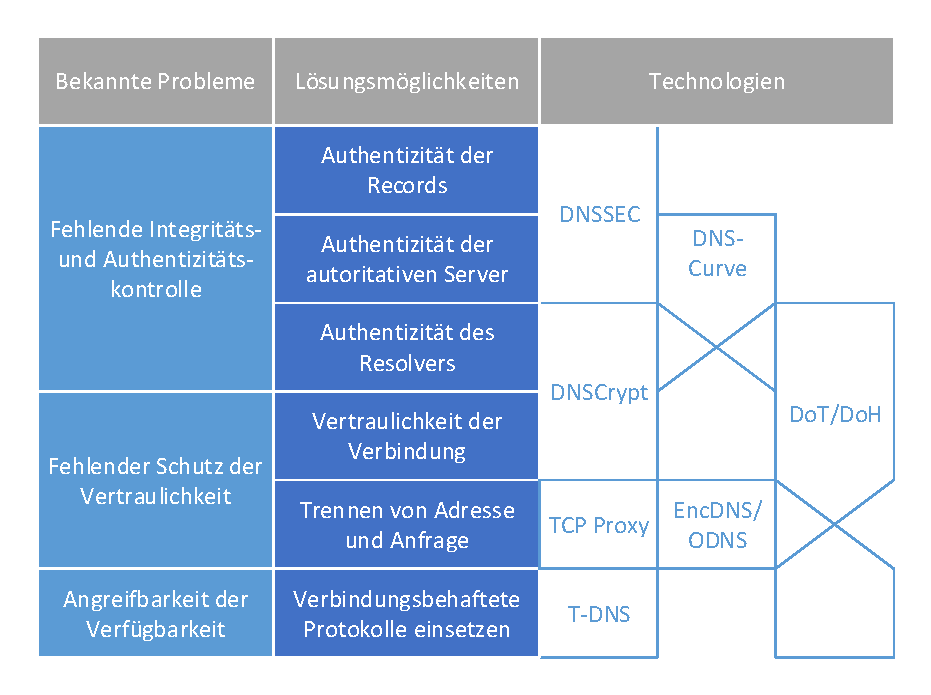
\includegraphics[width=0.7\textwidth]{Overview_Tecs}
    \caption{Darstellung des Bezugs zwischen DNS-Security Problemen, Lösungsmöglichkeiten und den bestehenden Technologien zur Umsetzung der Lösungen}
    \label{img:technologies-summary}
\end{figure}